\section{Spielstart} \label{sec:spielstart}
Sobald der erste verbundene Spieler ein Spiel ausgesucht hat, indem er darauf geklickt hat, und die Gruppengröße für das Spiel in Ordnung ist, wird die ID des Spieles an den Server geschickt.
Dieser sucht sich sowohl die Downloadlinks für die Client-Dateien, als auch für seine eigenen Server-Dateien. Anschließend überprüft er, ob das Spiel schon alle nötigen Dateien für die aktuelle Version heruntergeladen hat. Falls nicht wird das nachgeholt und anschließend werden die Download URLs für die Clients an alle verbundenen Spieler geschickt. Diese überprüfen auch deren Existenz und laden fehlende herunter. Verfügt ein Client über alle Dateien, so schickt er ein „ok“ an den Server. Sobald der Server Bestätigungen aller Clients erhalten hat, startet er seine Szene. Und schickt ein „ok“ an alle Clients, worauf hin diese auch deren Szenen starten. Dieser Ablauf ähnelt dem zwei Phasen Commit bei verteilten Datenbanken, wodurch die Sicherheit dieses Systems bewiesen ist.
\begin{figure}
    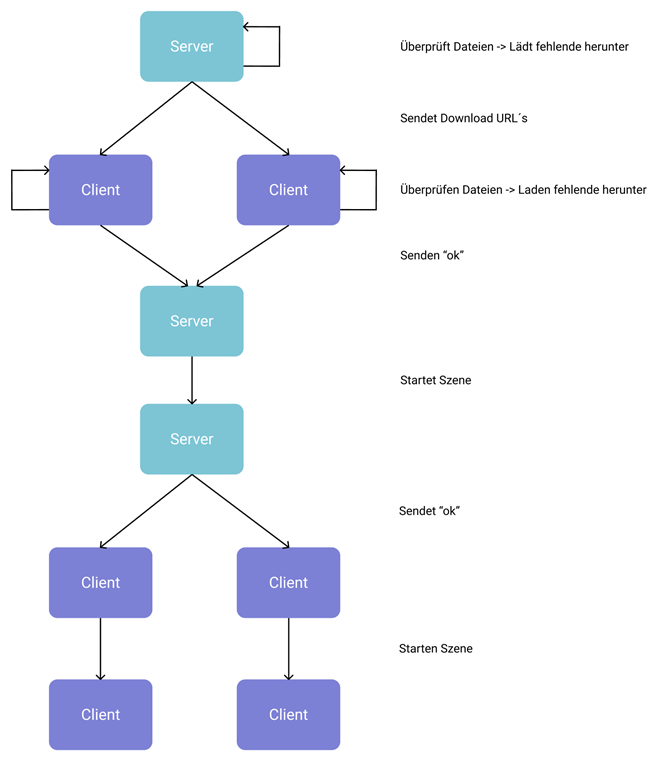
\includegraphics{images/spielstart.png}
    \caption{Vorgang bei Spielstart}
    \label{img:spielstart}
\end{figure}
\subsection{Probleme}
Spiele bestehen drei Komponenten, die gemeinsam dafür sorgen, dass die Spiele funktionieren. Sie bestehen aus Szenen, Modellen und Scripts. Szenen und Modelle, auch Texturen, Materialien, usw. sind in sogenannten „Assetbundles“ gespeichert. Alle Szenen des Clients sind in so einem „Assetbundle“ zusammengespeichert, ähnlich einer Zip-File. Alle Szenen des Server sind ebenfalls so persistiert. Die Unterscheidung zwischen Client und Server ist zwar nicht zwingend nötig, jedoch ist es Ressourcenverschwendung, wenn der Server auch Szenen der Clients speichert, da er diese ohnehin nicht startet, und umgekehrt. Die selbe Speicherung gilt für alle Modelle. Der Grund für die Trennung zwischen Client und Server bleibt gleich, jedoch wäre es deutlich einfacher, wenn Clientszenen und Clientmodelle zusammen gespeichert werden und alle Serverszenen und Servermodelle ebenfalls. Leider unterstützen „Assetbundles“ in Unity diese Funktionalität nicht. 
Als dritter Baustein gelten die Scripts, in denen die Logik der Spiele, das eigentliche Programm, beschrieben ist. Scripts können nicht zu „Assetbundles“ gemacht werden, jedoch gibt es unter Android und Windows die Möglichkeit, sie zu bündeln und dann zur Laufzeit eines Spieles zu verwenden. Unter Ios ist eine derartige Methode nicht möglich, da kein externer Code zur Laufzeit von Apps hinzugefügt werden kann oder darf. Diesen Sicherheitsmechanismus wird Apple nicht entfernen, was bedeutet, dass jeder Code immer in der App vorhanden sein muss. Für den Workflow des Erstellens eines neuen Spieles würde das bedeuten, dass wir alle verwendeten Scripts in das Hauptprojekt transferieren müssen und dann eine neue App Version in den App Store hochladen müssen. Apple User sind ein großer Anteil an unserer Zielgruppe, weswegen ein Ausschluss der Plattform nicht möglich ist. Zwei Speichervarianten für zwei Plattformen, wäre undenkbarer Mehraufwand, weshalb wir uns entschlossen, dass wir für jedes neue Spiel ein Update mit dessen Scripts für alle Plattformen herausbringen.
\subsection{Optimierungsansätze}
Der Fileserver von Firebase hat mit unserem Gratisbezahlplan eine maximale Downloadgröße und eine Grenze für Downloads pro Tag unabhängig von der Größe der Dateien, die heruntergeladen werden. Das ist der Grund, warum nur so viele Zugriffe gemacht werden sollten, wie nötig. Eine Maßnahme war es, dass der Server alle Download URLs beschafft und an die Clients weitergibt. Dieses Prinzip wurde auch für den eigentlichen Download selbst getestet. Im konkreten bedeutet das, dass der Server alle Plattformen der Clients überprüft und dann die Clientdateien für eben diese Plattformen herunterlädt, zwischenspeichert und anschließend den Clients über das lokale Netzwerk sendet. Dieser Ansatz entlastet den Fileserver, da dieser nur einen Downloadrequest verarbeiten muss, der Rest passiert nur zwischen den Spielern. Die gesamte Downloadzeit steigt jedoch dadurch, dass Dateien zwei Mal pro Spieler heruntergeladen werden, anstatt einmal und Clients können während dieser Zeit nur eingeschränkt kommunizieren, weshalb wir uns für die oben beschriebene Variante entschieden.